%---------- COURSE INFORMATION ------------------------
\newcommand{\course}{CIS 289-01}
\newcommand{\coursetitle}{INTRODUCTION TO HUMAN-COMPUTER INTERACTION/ \\ \hspace*{.4in}USER EXPERIENCE}
\newcommand{\courseloc}{Keller 234}
\newcommand{\coursetime}{Tuesday/Thursday 12:30 p.m. - 1:45 p.m.}
\newcommand{\coursedesc}{An interdisciplinary course which explores the foundations of HCI/UX including applied design, diverse forms of communication, cognitive processes, and software development in the context of how people interact with computing systems for real world application.  Specifically, the course provides an introduction to HCI/UX dimensions of design, development, and user research.  Experts from relevant academic disciplines and industry provide an interactive and career-oriented environment.}

\newcommand{\coursesec}{01}
\newcommand{\coursecredithours}{3}
\newcommand{\courseprereq}{None.}
\newcommand{\coursedelmethod}{Traditional Classroom}

\newcommand{\courseobjectives}{\item Explain interaction design techniques and the benefits of using interaction design principles for software development.
	\item Use best practices to design an effective interface.
	\item Implement a well-designed interface.
	\item Effectively evaluate an existing interface.
}

\newcommand{\coursetopics}{\item Usability of Interactive Systems
	\item Guidelines, Principles, and Theories
	\item Managing Design Processes
	\item Evaluating Interface Designs
	\item Direct Manipulation and Virtual Environments
	\item Menu Selection, Form Fill-In, and Dialog Boxes
	\item Command and Natural Languages
	\item Interaction Devices
	\item Collaboration and Social Media Participation 
	\item Quality of Service
	\item Balancing Function and Fashion 
	\item User Documentation and Online Help
	\item Information Search 
	\item Information Visualization}
\newcommand{\coursegrades}{Subject Exams (3 exams @ 20\% each)\dotfillsmall 60\% \\
		Projects\dotfillsmall 30\% \\
		Quiz and Participation Average\dotfillsmall 10\% }
\newcommand{\coursetext}{
	\adjustbox{valign=c}{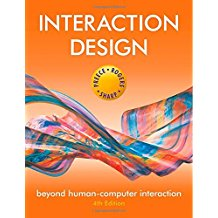
\includegraphics[width=1in]{img/cis289}} & \hangindent .4in \textbf{Textbook:} Preece, J., Sharp, H., Rogers, Y., Interaction Design: Beyond Human-Computer Interaction (4th Revised Edition). John Wiley \& Sons. ISBN-10: 1119020751, ISBN-13: 978-1119020752. \\
	%& \hangindent .4in Simulation Software: SAM 365 \& 2016 Assessments, Trainings, and Projects with MindTap Reader.
}